%!TEX root = ../dokumentation.tex
\chapter{Continuous Integration}\label{ch:continuous-integration}
Am Anfang des Projektes wurde \href{https://aws.amazon.com/de/codepipeline/}{AWS CodePipeline} als Continuous Integration (CI) verwendet. Dies stellte eine einfache Lösung dar, da unter anderem Github als Drittanbieter verfügbar ist. Somit wurde bei jeder Code-Änderung auf dem Master Branch des Github Repositories das neue Projekt auf den Server geladen.\\
Jedoch als später Tests mit PHPUnit hinzugefügt wurden, wurde vorausgesetzt, dass vor jedem Build das Projekt getestet wird.\\
Dazu wäre \href{https://aws.amazon.com/de/codebuild/}{AWS CodeBuild} eine Möglichkeit gewesen. Doch, da bereits persönlich mit dem kostenlosem CI Tool \href{https://travis-ci.com/}{Travis CI} gearbeitet wurde, fiel die Wahl auf dieses.

Für die Verwendung von Travis CI benötigt es die Berechtigung auf das Github Repository zuzugreifen. Außerdem muss eine \href{https://github.com/Drinkler/Planning-Poker/blob/master/.travis.yml}{\lstinline{.travis.yml}} Datei im Root des Repositories liegen. In dieser yml-Datei werden die \href{https://docs.travis-ci.com/user/job-lifecycle/}{nacheinander ablaufenden Befehle} definiert. In diesen Schritten wird das Projekt gebaut und getestet. Schlägt der Build fehl, wird er abgebrochen und der Code wird nicht auf den Server geladen. Durch die Möglichkeit mit \href{https://docs.travis-ci.com/user/deployment/codedeploy/}{AWS CodeDeploy} wird das Projekt automatisch, nach einem erfolgreichem Build, hochgeladen.\\
Travis CI klont das Repository in eine neue virtuelle Umgebung und führt diesen Build aus. Der letzte Build des Projektes ist \href{https://travis-ci.com/github/Drinkler/Planning-Poker}{hier} zu finden.\\
Um keine Anmeldedaten des Deploy Schrittes im Quellcode stehen zu haben, wurden die \href{https://docs.travis-ci.com/user/environment-variables/}{Travis CI Umgebungsvariablen} verw endet.

Die Abbildung \ref{ci} zeigt den Ablauf zwischen den einzelnen Schritten von der Entwicklung bis zur Veröffentlichung. Ein lokales Git repräsentiert einen Entwickler. Dies ist für andere Projekte variierbar.

\begin{figure}[H]
	\centering
  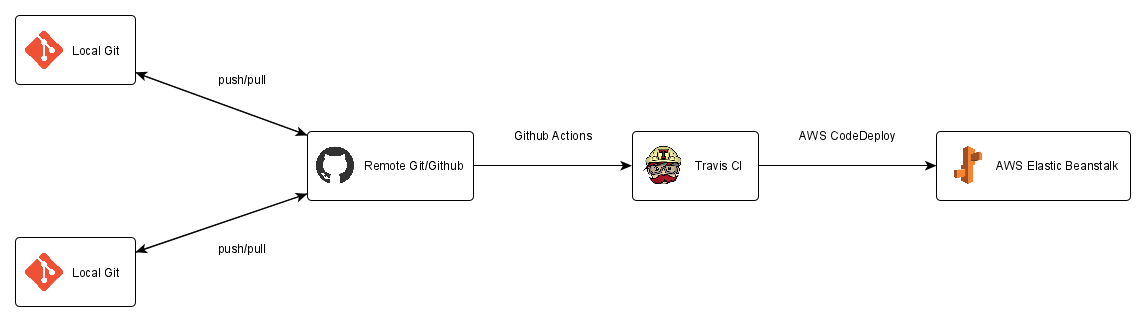
\includegraphics[width=\textwidth]{images/continuous_integration.png}
	\caption{Continuous Integration Prozess}
	\label{ci}
\end{figure}